\documentclass[margin=10pt]{standalone}
\usepackage{pgfplots}
\pgfplotsset{compat=newest}

\usepackage{palatino}
\newlength{\mainwidth}
\setlength{\mainwidth}{440pt}

\definecolor{color1}{HTML}{1b9e77}
\definecolor{color2}{HTML}{d95f02}
\definecolor{color3}{HTML}{7570b3}
\definecolor{color4}{HTML}{e7298a}
\definecolor{color5}{HTML}{66a61e}
\definecolor{color6}{HTML}{a6761d}
\definecolor{color7}{HTML}{e6ab02}

\begin{document}
\pgfplotsset{
    cycle list={
        {color1, mark=*, line width=1.5pt},
        {color2, mark=square*, line width=1.5pt},
        {color3, mark=triangle*, line width=1.5pt},
        {color4, mark=diamond*, line width=1.5pt},
        {color5, mark=pentagon*, line width=1.5pt},
        {color6, mark=o, line width=1.5pt},
        {color7, mark=star*, line width=1.5pt},
    }
}
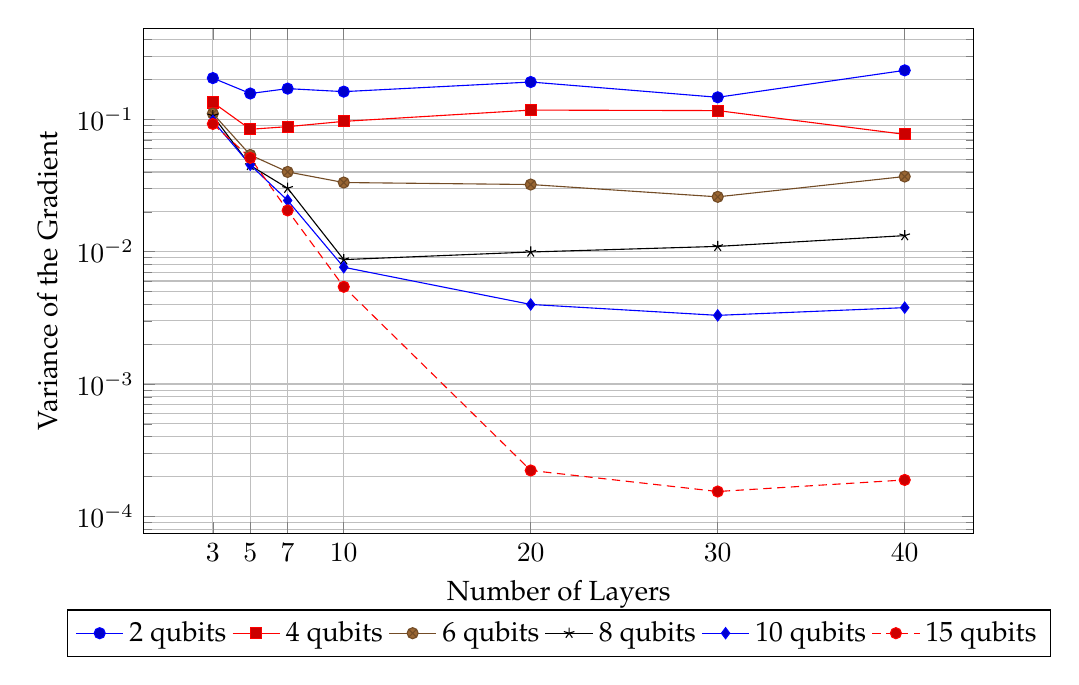
\begin{tikzpicture}
\begin{semilogyaxis}[
    xlabel={Number of Layers},
    ylabel={Variance of the Gradient},
    xtick={3, 5, 7, 10, 20, 30, 40},
    legend style={at={(0.5,-0.15)},anchor=north,legend columns=-1},
    grid=both,
    width=\textwidth,
    height=8cm,
    log basis y={10},
]

\addplot coordinates {(3, 0.20479486882686615) (5, 0.15661674737930298) (7, 0.17049561440944672) (10, 0.16179880499839783) (20, 0.191278338432312) (30, 0.1466093510389328) (40, 0.23431293666362762)};
\addlegendentry{2 qubits}

\addplot coordinates {(3, 0.13412517309188843) (5, 0.084050752222538) (7, 0.08797784894704819) (10, 0.09644491970539093) (20, 0.11735130846500397) (30, 0.11633412539958954) (40, 0.07697224617004395)};
\addlegendentry{4 qubits}

\addplot coordinates {(3, 0.11050938814878464) (5, 0.053772248327732086) (7, 0.04002636298537254) (10, 0.03328421711921692) (20, 0.03214666619896889) (30, 0.025948304682970047) (40, 0.036957789212465286)};
\addlegendentry{6 qubits}

\addplot coordinates {(3, 0.10643060505390167) (5, 0.044809721410274506) (7, 0.030151154845952988) (10, 0.008707592263817787) (20, 0.009939974173903465) (30, 0.010955099947750568) (40, 0.013214285485446453)};
\addlegendentry{8 qubits}

\addplot coordinates {(3, 0.09737081080675125) (5, 0.04525403305888176) (7, 0.024361632764339447) (10, 0.007621129974722862) (20, 0.003991606645286083) (30, 0.0033018237445503473) (40, 0.003775219200178981)};
\addlegendentry{10 qubits}

\addplot coordinates {(3, 0.09227895736694336) (5, 0.05115284025669098) (7, 0.02048601023852825) (10, 0.005426320247352123) (20, 0.0002221902832388878) (30, 0.00015407108003273606) (40, 0.00018841018027160317)};
\addlegendentry{15 qubits}

\end{semilogyaxis}
\end{tikzpicture}

\end{document}
